\documentclass{Class/julia}

\usepackage{geometry}
\usepackage{graphicx} % To use \resizebox
\usepackage{array} % For custom column widths
\usepackage{calc} % To use \widthof

\usepackage{siunitx} % Formatting numbers in a table

\usepackage{amsmath}
\usepackage{amsfonts}
\usepackage{subcaption}
\usepackage{threeparttable}
\usepackage{hyperref}
\usepackage{listings}
\usepackage{xcolor}
\usepackage{multirow}
%\usepackage{placeins}
\usepackage{booktabs}
\usepackage{tablefootnote}

\geometry{
    a4paper,
    total={170mm,257mm},
    left=20mm,
    top=20mm,
}

%\author{Julia Maria Wdowinska}
\date{} % Remove date from the title

\begin{document}

\begin{titlepage}
    \centering
    \vfill
    {\scshape\Large University of Milan \par}
    \vspace{0.5cm}
    {\scshape\large Faculty of Political, Economic and Social Sciences \par}
    \vspace{3cm}
    {\huge
    \textbf{A Bayesian Approach to Aggregate Insurance Claim Modeling} \\
    \vspace{0.5cm}
    \large Final Project in the Subject Bayesian Analysis \par}
    \vspace{2cm}
    {\large \textbf{Julia Maria Wdowinska} (43288A) \par}
    {\large \textbf{Edoardo Zanone} (33927A) \par}
    \vspace{0.5cm}
    {\large Data Science for Economics \par}
    {\large II Year \par}
    {\large Master’s Degree \par}
    \vfill
\begin{center}
\begin{figure}[h!]\centering
 
\includegraphics[keepaspectratio=true,scale=0.2]{logo} \\
\end{figure}
\end{center}
\vfill
\begin{center}
{\small{We declare that this material, which we now submit for assessment, is entirely our own work and has not been taken from the work of others, save and to the extent that such work has been cited and acknowledged within the text of our work. We understand that plagiarism, collusion, and copying are grave and serious offences in the university and accept the penalties that would be imposed should I engage in plagiarism, collusion or copying. This assignment, or any part of it, has not been previously submitted by us or any other person for assessment on this or any other course of study.}}
\end{center}
\vfill
    {\large \today \par}
    \vfill
\end{titlepage}

\tableofcontents
%\newpage

\section{Introduction}

In insurance modeling, accurately estimating the aggregate value of claims is essential for premium calculation, risk assessment, and maintaining solvency of insurance providers. The aggregate claim value refers to the total amount paid out for claims over a specified period. This quantity is typically modeled using a compound distribution, which separately describes the frequency and severity of claims. The frequency component, representing the number of claims within the period, is often modeled using a Poisson distribution. The severity component, which captures the magnitude of individual claims, is commonly modeled using heavy-tailed distributions such as the Pareto or Gamma distributions.

The traditional framework for modeling such processes is grounded in frequentist statistics. In this approach, the parameters of the underlying distributions—such as the Poisson rate parameter \( \lambda \), or the shape and scale pa- rameters \( \alpha \) and \( \beta \) of the Pareto distribution—are considered fixed but unknown quantities. These parameters~are typically estimated from observed data using techniques such as maximum likelihood estimation (MLE).

In contrast, the Bayesian framework treats these parameters as random variables characterized by prior~distributions. This allows for the incorporation of prior knowledge or beliefs about the parameters before any~data is observed. The prior distribution is updated using Bayes' theorem upon observing data, resulting in a posterior distribution that reflects the updated beliefs. This posterior distribution forms the basis for inference and pre- diction.

Bayesian methods offer significant advantages in insurance modeling. They are well-suited for incorporating expert knowledge or external information, handling limited or noisy datasets, and accommodating complex hier- archical structures commonly found in insurance data. Moreover, Bayesian inference provides a coherent frame- work for uncertainty quantification by yielding full posterior distributions over model parameters.

Nevertheless, Bayesian methods also come with certain limitations. The choice of prior distribution can~introduce subjectivity, and computational complexity can be significant, especially in models with high dimensionality or non-conjugate priors. Despite these challenges, the flexibility and robustness of the Bayesian framework make it a valuable approach for modeling aggregate insurance claims.

\section{Replication of \citet{dudley2006bayesian}}

Building on the theoretical background, this project aims to replicate the Bayesian modeling approach proposed by \citet{dudley2006bayesian}. The analysis is based on a dataset of automobile insurance claims exceeding 1.5 million, col- lected over a five-year period. The data, originally reported by \citet{rytgaard1990pareto}, is presented in Table \ref{tab:1}.

\begin{table}[!ht]
\centering
\footnotesize
\setlength{\tabcolsep}{5pt}
\caption{Insurance Claim Amounts Exceeding 1.5 Million (Data from \citealp{rytgaard1990pareto})}
\label{tab:1}
\begin{threeparttable}
\begin{tabular}{
>{\raggedright\arraybackslash}p{\widthof{Year}}
*{5}{S[table-format=2.3]}
}
\hline
\textbf{Year} & \multicolumn{5}{c}{\textbf{Claim Amounts (in millions)}} \\ \hline
1 & 2.495 & 2.120 & 2.095 & 1.700 & 1.650 \\
2 & 1.985 & 1.810 & 1.625 & \textendash & \textendash \\
3 & 3.215 & 2.105 & 1.765 & 1.715 & \textendash \\
4 & \textendash & \textendash & \textendash & \textendash & \textendash \\
5 & 19.180 & 1.915 & 1.790 & 1.755 & \textendash \\ \hline
\end{tabular}
\begin{tablenotes}
\footnotesize
\item The threshold of 1.5 million corresponds to the retention level of an excess-of-loss insurance policy\tablefootnote{To manage risk exposure, insurers frequently employ reinsurance strategies, which help reduce their financial liability on large claims. Under such arrangements, if a claim amount \( y \) exceeds a predetermined threshold \( d \) (the retention), the insurer is responsible only for paying up to \( d \), while any excess \( y - d \) is covered by the reinsurer.}.
\end{tablenotes}
\end{threeparttable}
\end{table}

\subsection{Model Specification}

To model this dataset within a Bayesian framework, assumptions about the distributions of both the number of claims in year \( t \) (\( N_t \)) and the amount of the \( i \)-th claim in year \( t \) (\( Y_{i,t} \)) were necessary. Claims were assumed to occur randomly and independently at a constant rate over time, so \( N_t \) was modeled using a Poisson distribution. A Pareto distribution was selected for \( Y_{i,t} \), as a heavy-tailed loss distribution was needed to account for the fact that individual claim amounts are positive and may include large outliers. That is,
\begin{align*}
N_t &\sim \text{Poisson}(\theta), \quad 0 < \theta < \infty, \\
Y_{i,t} &\sim \text{Pareto}(\alpha, \beta), \quad \alpha > 0, \quad 0 < \beta < y.
\end{align*}

\noindent The \text{Pareto}\((\alpha, \beta)\) distribution with support \( [\beta, \infty) \) was particularly suitable in this context, as it was employed to model claim amounts exceeding a specified threshold.

In addition, the following assumptions were made:

\begin{itemize}
\item \( N_t \) are independently and identically distributed (i.i.d.) across \( t \),
\item \( Y_{i,t} \) are i.i.d.\ across both \( i \) and \( t \),
\item \( N_t \) and \( Y_{i,t} \) are independent for all \( i \) and \( t \).
\end{itemize}

\noindent Under these assumptions, the aggregate claim amount in year \( t \) was defined as
\[
S_t = Y_{1,t} + Y_{2,t} + \cdots + Y_{N_t,t}.
\]

Next, prior distributions for the parameters \( \alpha \), \( \beta \), and \( \theta \) were specified. Due to limited prior knowledge about their true values—beyond the assumption that they are strictly positive—vague Gamma priors\footnote{Each of these Gamma priors has a variance of \(10^8\), implying minimal prior influence so that most of the information about~the parameters is derived from the dataset. Additionally, the Gamma distribution is conjugate to both the Poisson and Pareto likeli- hoods, facilitating analytical tractability in Bayesian inference.} were chosen:
\[
\alpha \sim \text{Gamma}(1, 0.0001), \quad \beta \sim \text{Gamma}(1, 0.0001), \quad \theta \sim \text{Gamma}(1, 0.0001),
\]
with the constraint \( 0 < \beta < \min\{y_{i,t}\} \) to ensure validity of the Pareto distribution.

Finally, the posterior distributions were derived. First, the joint posterior distribution of \( (\alpha, \beta) \) was obtained via Bayes' theorem\footnote{Here, assuming that \( \alpha \) and \( \beta \) are independent, the joint prior \( \pi(\alpha, \beta) \) was computed as \( \pi(\alpha) \cdot \pi(\beta) \).}:
\begin{align*}
\pi(\alpha, \beta \mid \mathbf{y}) &\propto \pi(\alpha) \cdot \pi(\beta) \cdot f(\mathbf{y} \mid \alpha, \beta) \\
&\propto 0.0001 \cdot \exp(-0.0001 \alpha) \cdot 0.0001 \cdot \exp(-0.0001 \beta) \cdot \prod_{i=1}^{n} \frac{\alpha \beta^\alpha}{y_i^{\alpha+1}} \\
&\propto \exp(-0.0001 \alpha) \cdot \exp(-0.0001 \beta) \cdot \alpha^n \cdot \beta^{n \alpha} \left( \prod_{i=1}^{n} y_i \right)^{-(\alpha + 1)} \\
&\propto \alpha^n \cdot \exp(-0.0001 \alpha) \cdot \left( \prod_{i=1}^{n} y_i \right)^{-\alpha} \cdot \beta^{n \alpha} \cdot \exp(-0.0001 \beta) \\
&\propto \alpha^n \cdot \exp\left( - \left( 0.0001 + \sum_{i=1}^{n} \ln(y_i) \right) \alpha \right) \cdot \beta^{n \alpha} \cdot \exp(-0.0001 \beta)
\end{align*}

\noindent As a result, the full conditional posterior distributions of \( \alpha \) and \( \beta \) were as follows:
\begin{align*}
\pi(\alpha \mid \beta, \mathbf{y}) &\propto \alpha^n \cdot \exp\left( - \left( 0.0001 - n \ln(\beta) + \sum_{i=1}^{n} \ln(y_i) \right) \alpha \right), \\
\pi(\beta \mid \alpha, \mathbf{y}) &\propto \beta^{n \alpha} \cdot \exp(-0.0001 \beta),
\end{align*}

\noindent which implied that:
\begin{align*}
\alpha \mid \beta, \mathbf{y} &\sim \text{Gamma}\left(n+1, \sum_{i=1}^{n} \ln(y_i) - n \ln(\beta) + 0.0001\right), \\
\beta \mid \alpha, \mathbf{y} &\sim \text{Gamma}(n \alpha + 1, 0.0001).
\end{align*}

Similarly, the posterior distribution of \( \theta \) was obtained via Bayes' theorem:
\begin{align*}
\pi(\theta \mid \mathbf{n}) &\propto \pi(\theta) \cdot f(\mathbf{n} \mid \theta) \\
&\propto \exp(-0.0001 \theta) \cdot \prod_{t=1}^{T} \left( \theta^{n_t} \cdot \exp(-\theta) \right) \\
&\propto \exp(-0.0001 \theta) \cdot \theta^{\sum_{t=1}^{T} n_t} \cdot \exp(-5 \theta) \\
&\propto \exp(-5.0001 \theta) \cdot \theta^{\sum_{t=1}^{T} n_t}
\end{align*}

\noindent which implied that:
\[
\theta \mid \mathbf{n} \sim \text{Gamma}\left( \sum_{t=1}^{T} n_t + 1, 5.0001 \right)
\]

\subsection{Sampling Results}

Since all three posterior distributions were standard distributions, the Gibbs sampling method was employed to draw realizations from them\footnote{Markov Chain Monte Carlo (MCMC) methods, like Gibbs sampling, are used to draw samples from intractable posterior distributions. Gibbs sampling is efficient when full conditional posteriors are in closed form, often with conjugate priors. When posteriors are not in closed form, the Metropolis-Hastings algorithm can be used to generate candidate values from a proposal~distribution.}. This was implemented using the \texttt{JAGS} program, which was called from within~\texttt{R}. Following \citet{dudley2006bayesian}, three Markov chains were run in parallel. The initial values of \( \alpha \), \( \beta \), and \( \theta \) were~chosen to be well-dispersed and are presented in Table~\ref{tab:2}.

\begin{table}[!ht]
\centering
\footnotesize
\setlength{\tabcolsep}{5pt}
\caption{Initial Parameter Values}
\label{tab:2}
\begin{threeparttable}
\begin{tabular}{
>{\raggedright\arraybackslash}p{\widthof{Chain}}
*{3}{S[table-format=6.5]}
}
\hline
\textbf{Chain} & \( \alpha \) & \( \beta \) & \( \theta \) \\ \hline
1 & 0.00001 & 0.00001 & 0.00001 \\
2 & 100000 & 1 & 100000 \\
3 & 3.076 & 1.625 & 3.200 \\ \hline
\end{tabular}
\begin{tablenotes}
\footnotesize
\item These values are taken from \citet{dudley2006bayesian}.
\end{tablenotes}
\end{threeparttable}
\end{table}

A burn-in of 20,000 iterations was used. The statistics computed from the subsequent 30,000 iterations are presented in Table~\ref{tab:3}. A comparison with those reported by \citet{dudley2006bayesian} shows a close match, indicating that the model was properly specified and the Gibbs sampler executed correctly.

\begin{table}[!ht]
\centering
\footnotesize
\setlength{\tabcolsep}{5pt}
\caption{Posterior Statistics}
\label{tab:3}
\begin{threeparttable}
\begin{tabular}{
>{\raggedright\arraybackslash}p{\widthof{\( \mathbb{E}[y] \)}}
*{2}{S[table-format=1.3]}
>{\raggedright\arraybackslash}p{\widthof{\textbf{95\% Bayesian Credible Interval}}}
}
\hline
 & \textbf{Mean} & \textbf{Standard Deviation} & \textbf{95\% Bayesian Credible Interval} \\ \hline
\( \alpha \) & 3.076 & 0.762 & (1.762, 4.752) \\
\( \beta \) & 1.591 & 0.035 & (1.498, 1.624) \\
\( \theta \) & 3.399 & 0.820 & (1.986, 5.185) \\
\( \mathbb{E}[y] \) & 2.507 & 1.071 & (2.024, 3.637) \\ \hline
\end{tabular}
\begin{tablenotes}
\footnotesize
\item \( \mathbb{E}[y] \) was calculated for each simulated set of parameters \( \alpha \) and \( \beta \), and from these values, the mean, standard deviation, and 95\% Bayesian credible interval were subsequently computed.
\end{tablenotes}
\end{threeparttable}
\end{table}

In addition, density plots were generated for each of the parameters and for \( \mathbb{E}[y] \), as presented in Figure~\ref{fig:1}. The resulting densities for the parameters resemble Gamma distributions, with the density of \( \beta \) appropriately truncated at \( \min\{y_{i,t}\} = 1.625 \). The plot for \( \mathbb{E}[y] \) displays a right-skewed distribution that permits very large values, albeit with very low probability---consistent with expectations.

\begin{figure}[!ht]
    \centering
    \caption{Posterior Densities}
    \label{fig:1}
    \begin{minipage}{0.45\textwidth}
        \centering
        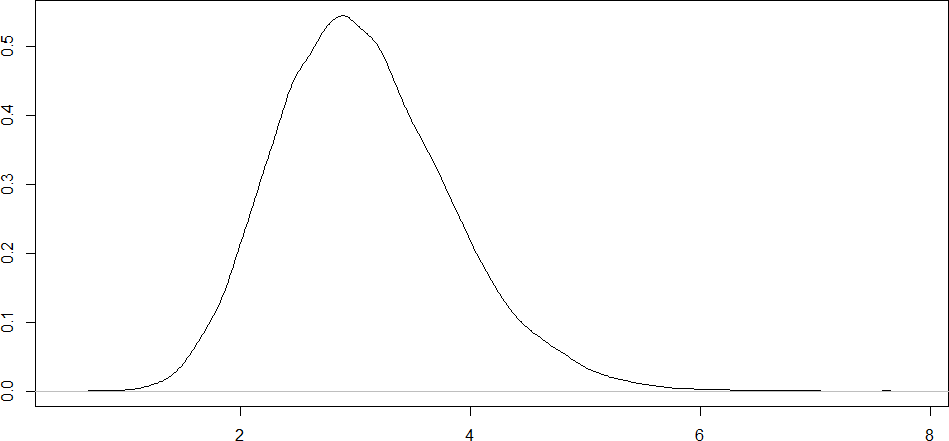
\includegraphics[width=\textwidth]{rytgaard1990/density_alpha.png}
        \subcaption{\( \alpha \)}
    \end{minipage}%
    \hfill
    \begin{minipage}{0.45\textwidth}
        \centering
        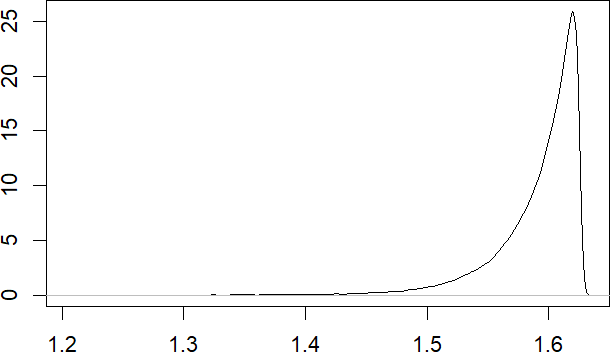
\includegraphics[width=\textwidth]{rytgaard1990/density_beta.png}
        \subcaption{\( \beta \)}
    \end{minipage} \\
    
    \vspace{0.5cm}
    
    \begin{minipage}{0.45\textwidth}
        \centering
        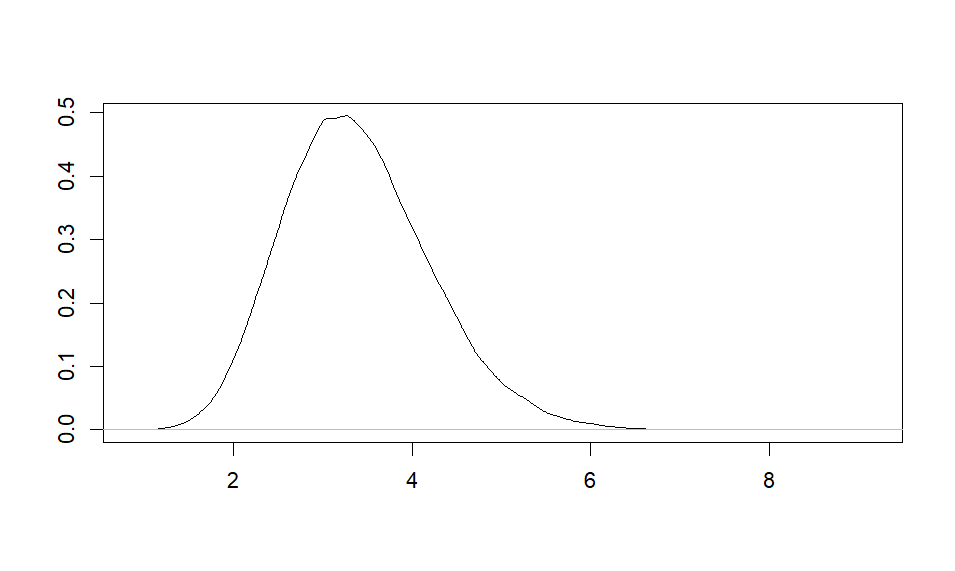
\includegraphics[width=\textwidth]{rytgaard1990/density_theta.png}
        \subcaption{\( \theta \)}
    \end{minipage}%
    \hfill
    \begin{minipage}{0.45\textwidth}
        \centering
        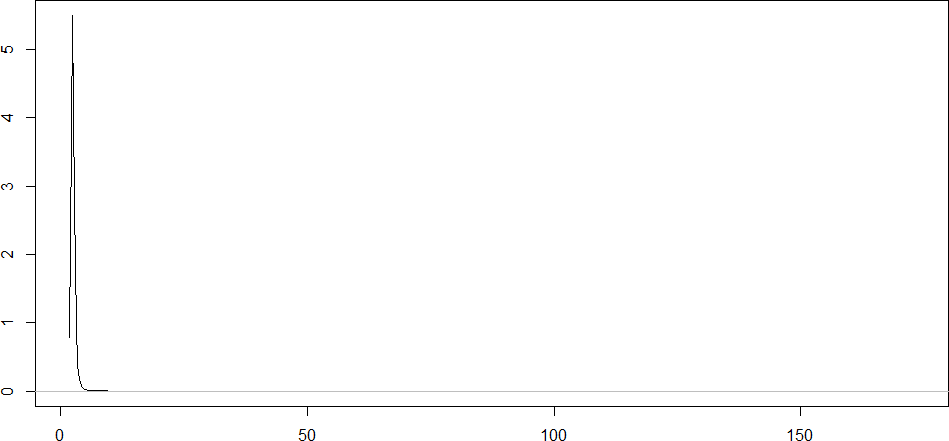
\includegraphics[width=\textwidth]{rytgaard1990/density_E_y.png}
        \subcaption{\( \mathbb{E}[y] \)}
    \end{minipage}
    
\end{figure}

The posterior means of \( \alpha \) and \( \beta \) were used as parameters of the Pareto distribution, and the corresponding cumulative distribution function (CDF) was plotted against the empirical cumulative data (\( y_{i,t} \)). Similarly, the posterior mean of \( \theta \) was used as the parameter of the Poisson distribution, and its CDF was plotted against the empirical cumulative data (\( n_t \)). The Pareto\((3.079,\,1.592)\) distribution provides a close fit to the empirical data. The Poisson\((3.396)\) distribution also fits the observed frequencies quite well (see Figures \ref{fig:2} and \ref{fig:3}).

\begin{figure}[!ht]
    \centering
    \caption{Empirical vs.\ Fitted Pareto CDF}
    \label{fig:2}
    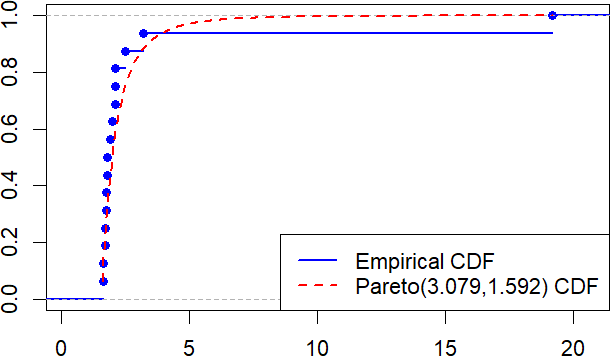
\includegraphics[width=.75\textwidth]{rytgaard1990/empirical_vs_pareto.png}
\end{figure}

\begin{figure}[!ht]
    \centering
    \caption{Empirical vs.\ Fitted Poisson CDF}
    \label{fig:3}
    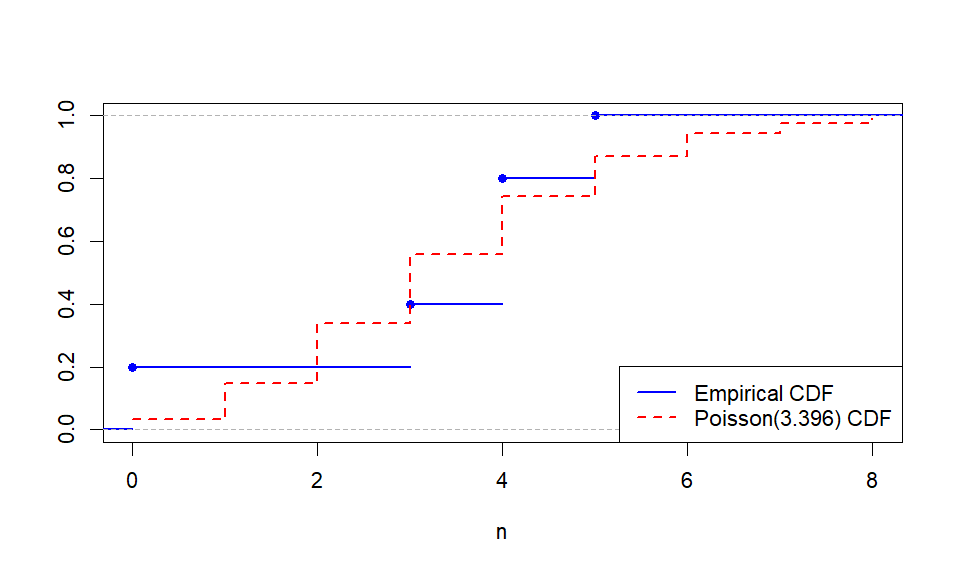
\includegraphics[width=.75\textwidth]{rytgaard1990/empirical_vs_poisson.png}
\end{figure}

\subsection{Convergence Diagnostics}

Throughout all computations above, it was assumed that the Markov chains had converged to a stationary~distribution after discarding the initial 20,000 iterations, following the approach of \citet{dudley2006bayesian}. However, it was essential to verify that convergence had indeed occurred. The first method of assessment involved visual inspec- tion\footnote{Visual inspection involves assessing how well a chain explores the parameter space. Poor mixing—where the chain moves slowly or gets stuck—indicates potential convergence issues. Trace plots help identify such problems by showing how sampled values evolve over iterations for each parameter.}. Figure~\ref{fig:4} presents trace plots for all three parameters, showing the sampled values across iterations. These plots indicate good mixing, suggesting that the chains have likely converged.

\begin{figure}[!ht]
    \centering
    \caption{Trace Plots}
    \label{fig:4}
    \begin{subfigure}{0.45\textwidth}
        \centering
        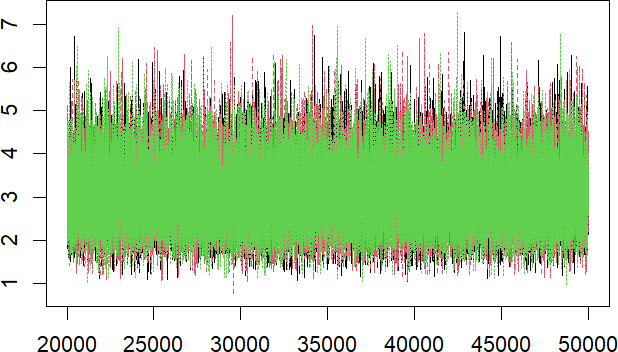
\includegraphics[width=\textwidth]{rytgaard1990/trace_alpha.png}
        \caption{\( \alpha \)}
    \end{subfigure}
    \hfill
    \begin{subfigure}{0.45\textwidth}
        \centering
        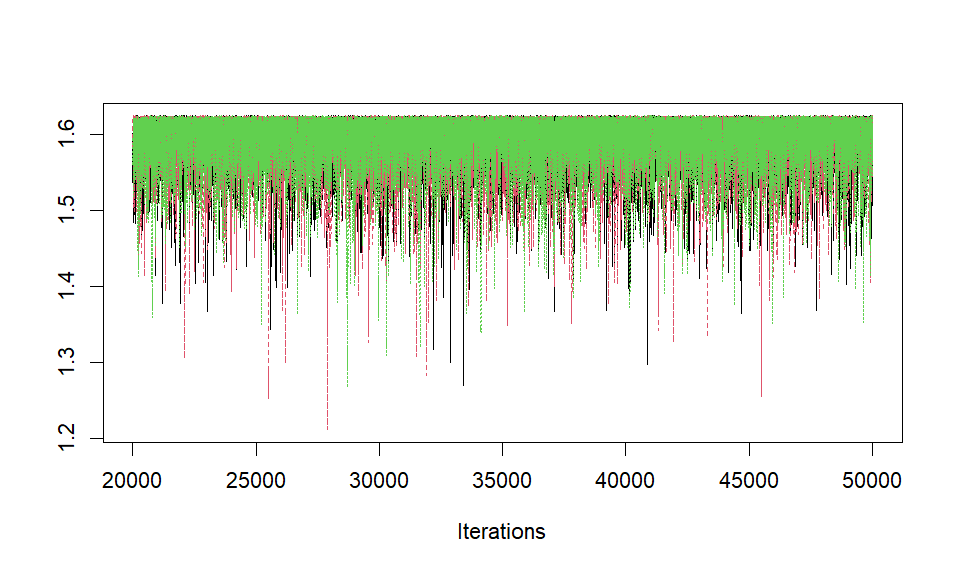
\includegraphics[width=\textwidth]{rytgaard1990/trace_beta.png}
        \caption{\( \beta \)}
    \end{subfigure}

    \vspace{1em}

    \begin{subfigure}{0.45\textwidth}
        \centering
        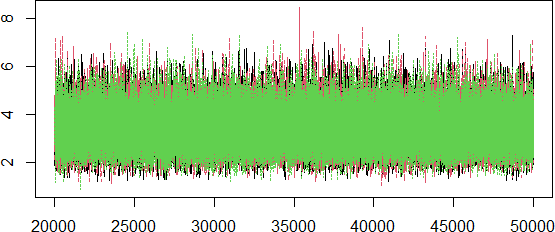
\includegraphics[width=\textwidth]{rytgaard1990/trace_theta.png}
        \caption{\( \theta \)}
    \end{subfigure}

\end{figure}

Convergence was further assessed using the Gelman--Rubin diagnostic \citep{Gelman1992}, applied to the post-burn-in iterations (20,001–50,000). The results, shown in Table~\ref{tab:4}, indicate that all univariate potential scale reduction factors (PSRFs) have point estimates and upper confidence bounds equal to 1. The multivariate PSRF is also 1. These values again suggest that the Markov chains have likely converged, both individually~and jointly.

\begin{table}[!ht]
\centering
\footnotesize
\caption{Potential Scale Reduction Factors (Gelman--Rubin Diagnostic)}
\label{tab:4}
\begin{threeparttable}
\begin{tabular}{
  >{\raggedright\arraybackslash}p{\widthof{\textbf{Multivariate PSRF}}}
  *{2}{S[table-format=1.2]}
}
\hline
\textbf{Parameter} & \textbf{Point Estimate} & \textbf{Upper C.I.} \\
\hline
\( \alpha \) & 1.00 & 1.00 \\
\( \beta \)  & 1.00 & 1.00 \\
\( \theta \) & 1.00 & 1.00 \\
\hline
\textbf{Multivariate PSRF} & \multicolumn{2}{c}{1.00} \\
\hline
\end{tabular}
\begin{tablenotes}
\footnotesize
\item The diagnostic was applied to iterations 20,001–50,000.
\end{tablenotes}
\end{threeparttable}
\end{table}

Figure~\ref{fig:5} shows how the univariate PSRF point estimates evolve with increasing iterations. Throughout all~iterations, all estimates remain below 1.1, which is commonly considered an acceptable threshold for convergence. This further confirms that the chains have likely reached a stable distribution.

\begin{figure}[!ht]
    \centering
    \caption{PSRF Values (Gelman--Rubin Diagnostic)}
    \label{fig:5}
    \begin{subfigure}{0.45\textwidth}
        \centering
        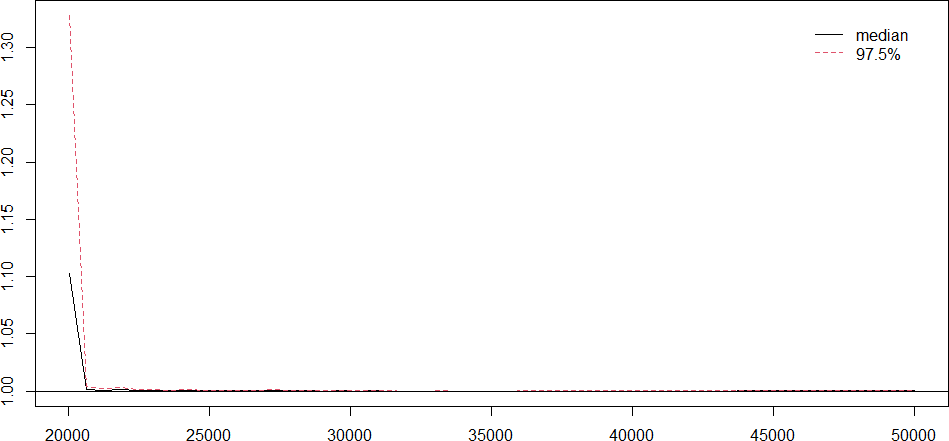
\includegraphics[width=\textwidth]{rytgaard1990/gelman_alpha.png}
        \caption{\( \alpha \)}
    \end{subfigure}
    \hfill
    \begin{subfigure}{0.45\textwidth}
        \centering
        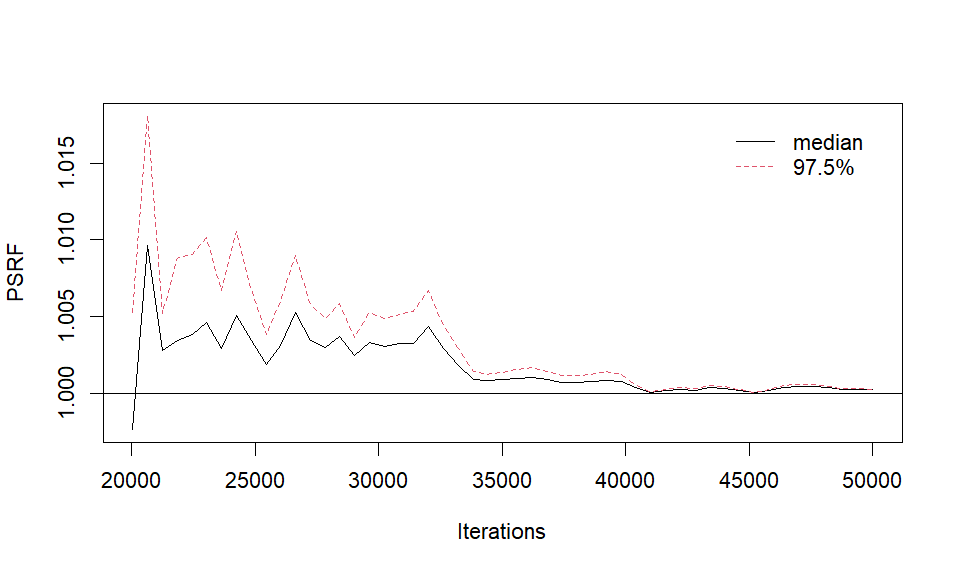
\includegraphics[width=\textwidth]{rytgaard1990/gelman_beta.png}
        \caption{\( \beta \)}
    \end{subfigure}

    \vspace{1em}

    \begin{subfigure}{0.45\textwidth}
        \centering
        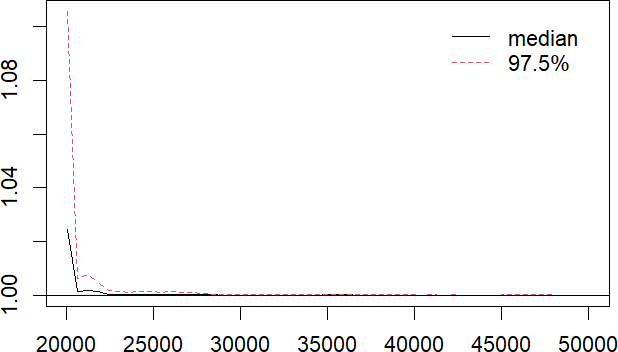
\includegraphics[width=\textwidth]{rytgaard1990/gelman_theta.png}
        \caption{\( \theta \)}
    \end{subfigure}
\end{figure}

In addition, autocorrelation\footnote{The autocorrelation function (ACF) shows the correlation between samples at different lags. High autocorrelation indicates strong dependence between draws, leading to slow mixing. Thinning reduces this dependence by keeping only every \( k \)th sample.} plots were generated for all three parameters (see Figure~\ref{fig:6}), and values at~lags 1 through 10 are reported in Table~\ref{tab:5}. Several high autocorrelations were observed, particularly for \( \beta \), which~motivated the use of a thinning interval of 10 iterations, as suggested by \citet{dudley2006bayesian}.

\begin{figure}[!ht]
    \centering
    \caption{Autocorrelation Plots}
    \label{fig:6}
    \begin{subfigure}{0.45\textwidth}
        \centering
        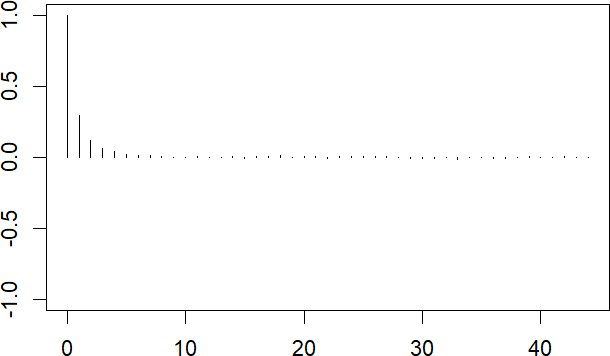
\includegraphics[width=\textwidth]{rytgaard1990/acf_alpha.png}
        \caption{\( \alpha \)}
    \end{subfigure}
    \hfill
    \begin{subfigure}{0.45\textwidth}
        \centering
        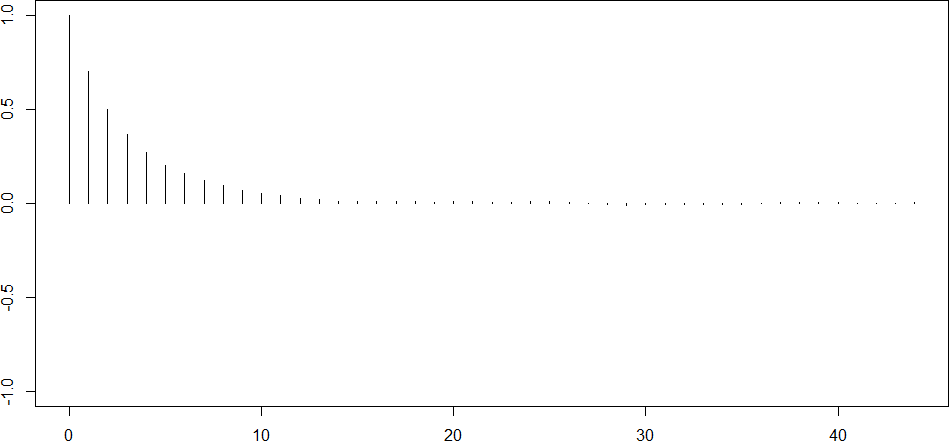
\includegraphics[width=\textwidth]{rytgaard1990/acf_beta.png}
        \caption{\( \beta \)}
    \end{subfigure}

    \vspace{1em}

    \begin{subfigure}{0.45\textwidth}
        \centering
        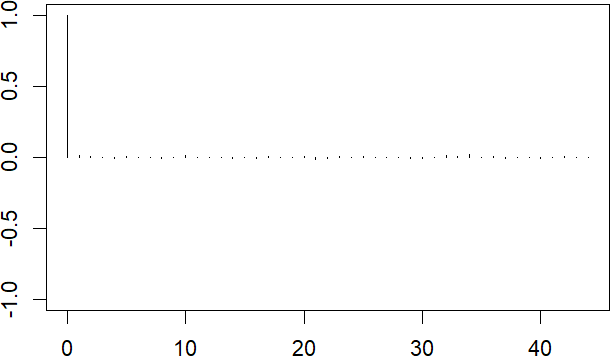
\includegraphics[width=\textwidth]{rytgaard1990/acf_theta.png}
        \caption{\( \theta \)}
    \end{subfigure}
\end{figure}

\begin{table}[!ht]
\centering
\footnotesize
\setlength{\tabcolsep}{5pt}
\caption{Autocorrelations at Lags 1--10}
\label{tab:5}
\begin{tabular}{
>{\raggedright\arraybackslash}p{\widthof{\textbf{Lag}}}
*{3}{S[table-format=-1.3]}
}
\hline
\textbf{Lag} & \( \alpha \) & \( \beta \) & \( \theta \) \\
\hline
1  & 0.288 & 0.699 & -0.001 \\
2  & 0.109 & 0.498 & -0.001 \\
3  & 0.053 & 0.356 & 0.003 \\
4  & 0.035 & 0.257 & -0.007 \\
5  & 0.019 & 0.191 & 0.002 \\
6  & 0.008 & 0.144 & -0.006 \\
7  & 0.010 & 0.104 & 0.003 \\
8  & 0.013 & 0.079 & -0.007 \\
9  & 0.007 & 0.061 & 0.001 \\
10 & 0.006 & 0.048 & 0.000 \\
\hline
\end{tabular}
\end{table}

Consequently, the chains were rerun with this thinning. Figure~\ref{fig:7} presents the corresponding trace plots, and Figure~\ref{fig:8} shows the updated autocorrelation plots. The trace plots indicate that the chains have mixed well,~and the autocorrelation plots demonstrate that all autocorrelation values at lags 1, 2, and beyond have~become~negligible.

\begin{figure}[!ht]
    \centering
    \caption{Trace Plots After Thinning}
    \label{fig:7}
    \begin{subfigure}{0.45\textwidth}
        \centering
        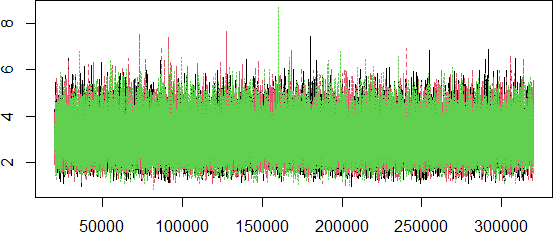
\includegraphics[width=\textwidth]{rytgaard1990/trace_after_thinning_alpha.png}
        \caption{\( \alpha \)}
    \end{subfigure}
    \hfill
    \begin{subfigure}{0.45\textwidth}
        \centering
        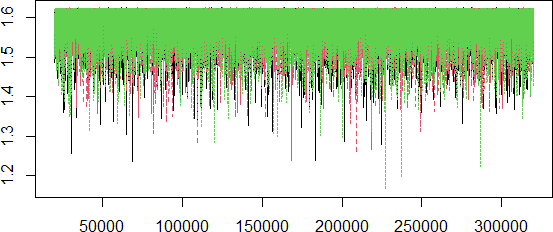
\includegraphics[width=\textwidth]{rytgaard1990/trace_after_thinning_beta.png}
        \caption{\( \beta \)}
    \end{subfigure}

    \vspace{1em}

    \begin{subfigure}{0.45\textwidth}
        \centering
        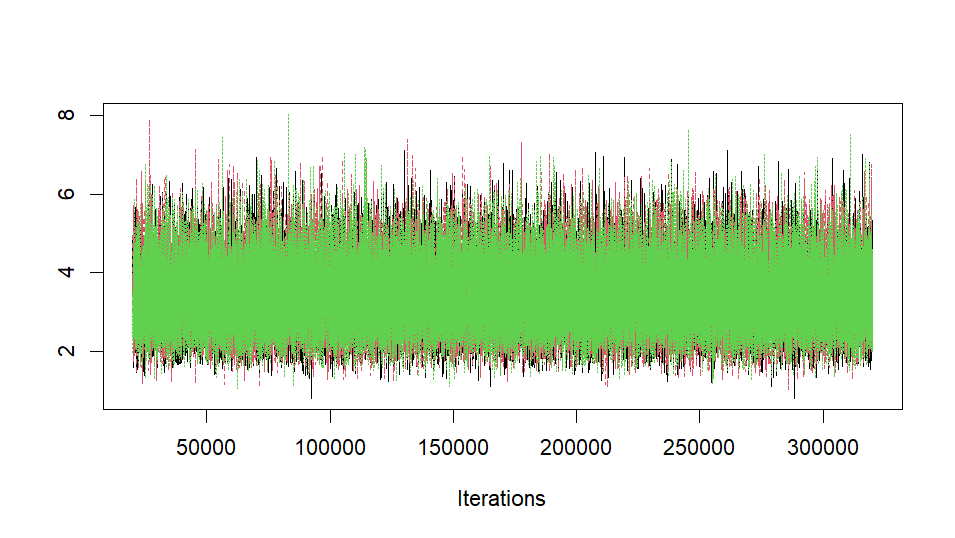
\includegraphics[width=\textwidth]{rytgaard1990/trace_after_thinning_theta.png}
        \caption{\( \theta \)}
    \end{subfigure}
\end{figure}

\begin{figure}[!ht]
    \centering
    \caption{Autocorrelation Plots After Thinning}
    \label{fig:8}
    \begin{subfigure}{0.45\textwidth}
        \centering
        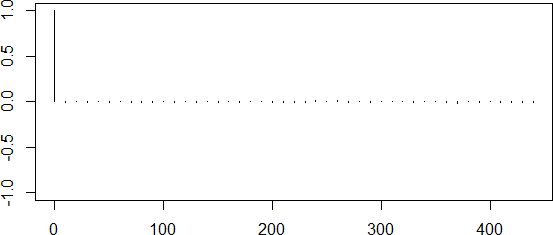
\includegraphics[width=\textwidth]{rytgaard1990/acf_after_thinning_alpha.png}
        \caption{\( \alpha \)}
    \end{subfigure}
    \hfill
    \begin{subfigure}{0.45\textwidth}
        \centering
        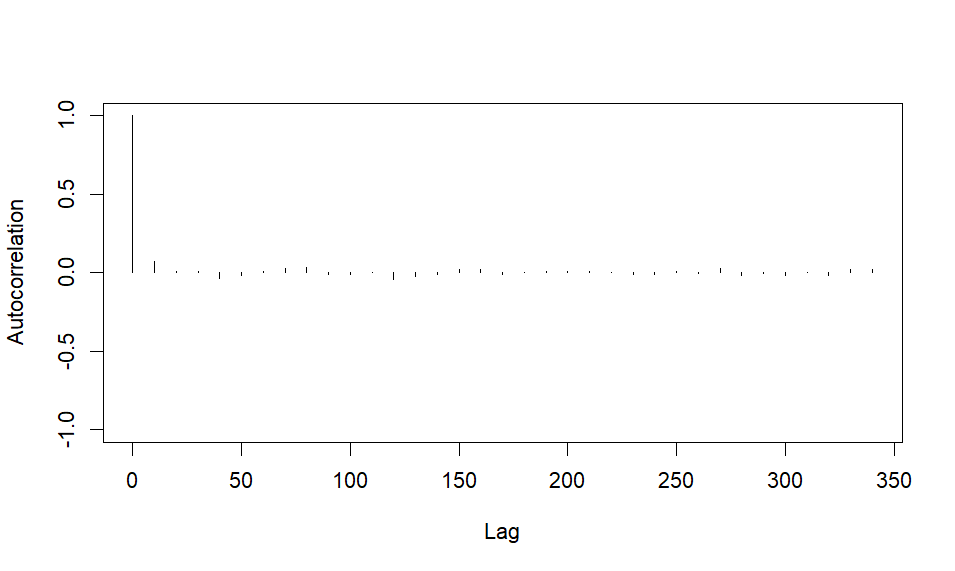
\includegraphics[width=\textwidth]{rytgaard1990/acf_after_thinning_beta.png}
        \caption{\( \beta \)}
    \end{subfigure}

    \vspace{1em}

    \begin{subfigure}{0.45\textwidth}
        \centering
        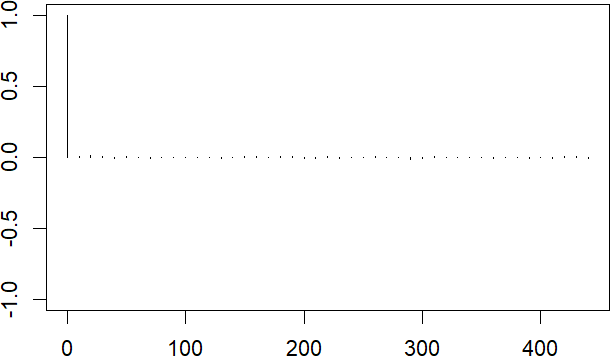
\includegraphics[width=\textwidth]{rytgaard1990/acf_after_thinning_theta.png}
        \caption{\( \theta \)}
    \end{subfigure}

\end{figure}

\subsection{Predictive Inference}

The ultimate objective of the analysis was to predict future values of \( S_t \), which was accomplished using the~posterior predictive distribution. For a variable \( z \), this distribution is defined as\footnote{This method accounts for the uncertainty in \( \boldsymbol{\phi} \) by integrating over its possible values, weighted by their posterior probabilities.}:
\[
\pi(z \mid \mathbf{y}) = \int_{\Theta} f(z \mid \mathbf{\phi}) \, \pi(\mathbf{\phi} \mid \mathbf{y}) \, d\mathbf{\phi}
\]

\noindent where \( \pi(\mathbf{\phi} \mid \mathbf{y}) \) is the posterior distribution of \( \mathbf{\phi} \), and \( f(z \mid \mathbf{\phi}) \) is the likelihood of \( z \) given \( \mathbf{\phi} \).

Let \( \mathbf{n} \) denote the observed data, and let \( N_f \) represent a future observation of \( N_t \). Then the posterior predic- tive distribution of \( N_f \) is given by:
\[
\begin{aligned}
p (N_f = n \mid \mathbf{n}) 
&= \int_0^{\infty} p(N_f = n \mid \theta) \pi(\theta \mid \mathbf{n}) \, d\theta \\
&= \mathbb{E}_{\theta \mid \mathbf{n}}\left[ p(N_f = n \mid \theta) \right] \\
&= \mathbb{E}_{\theta \mid \mathbf{n}}\left[ \frac{\theta^n e^{-\theta}}{n!} \right]
\end{aligned}
\]

\noindent Since the integral cannot be evaluated analytically, it is typically approximated using samples from the posterior distribution obtained via MCMC. Specifically, the expectation is approximated as:
\[
p (N_f = n \mid \mathbf{n}) \approx \frac{1}{m} \sum_{i=1}^{m} \frac{(\theta^{(i)})^n e^{-\theta^{(i)}}}{n!}
\]

\noindent where \( \theta^{(i)} \) is the \( i \)-th sample from the MCMC chain and \( m \) is the number of iterations after burn-in and thinning.

Similarly, let \( \mathbf{y} \) denote the observed data, and let \( Y_f \) represent a future observation of \( Y_{i,t} \). Then the posterior predictive cumulative distribution function (CDF) of \( Y_f \) is given by:
\[
\begin{aligned}
p (Y_f \leq y \mid \mathbf{y}) 
&= \int_{\mathbf{u}} p(Y_f \leq y \mid \mathbf{u}) \, \pi(\mathbf{u} \mid \mathbf{y}) \, d\mathbf{u} \\
&= \mathbb{E}_{\mathbf{u} \mid \mathbf{y}}\left[ p(Y_f \leq y \mid \alpha, \beta) \right]
\end{aligned}
\]

\noindent Again,
\[
p (Y_f \leq y \mid \mathbf{y}) \approx \frac{1}{m} \sum_{i=1}^{m} \left( 1 - \left( \frac{\beta^{(i)}}{y} \right)^{\alpha^{(i)}} \right)
\]

\noindent where \( \alpha^{(i)} \) and \( \beta^{(i)} \) denote the \( i \)-th samples from the MCMC chain.

Table~\ref{tab:6} shows the estimated probabilities of \( N_f = n \) for \( n = 0, \dots, 14 \), which are consistent with the findings of \citet{dudley2006bayesian}. Figure~\ref{fig:9} displays the estimated predictive probability density function (PDF) of \( Y_f \), obtained using the inverse CDF method\footnote{Specifically, 1,000 values \( U \sim \mathrm{Uniform}(0, 1) \) were generated. For each value, the transformation \(\beta^{(i)} (1 - U)^{-1/\alpha^{(i)}}\) was applied for each \( i \), and the results were averaged across \( i \). The resulting 1,000 values were then used to approximate the PDF of \( Y_f \) via~kernel density estimation (KDE).}.

\begin{table}[!ht]
\centering
\footnotesize
\setlength{\tabcolsep}{5pt}
\caption{Estimates of \( p (N_f = n \mid \mathbf{n}) \)}
\label{tab:6}
\begin{tabular}{
>{\raggedright\arraybackslash}p{\widthof{\textbf{n}}}
S[table-format=1.4]
}
\hline
\( n \) & \textbf{Probability} \\ 
\hline
0  & 0.0453 \\ 
1  & 0.1282 \\ 
2  & 0.1919 \\ 
3  & 0.2023 \\ 
4  & 0.1683 \\ 
5  & 0.1177 \\ 
6  & 0.0718 \\ 
7  & 0.0393 \\ 
8  & 0.0196 \\ 
9  & 0.0091 \\ 
10 & 0.0039 \\ 
11 & 0.0016 \\ 
12 & 0.0006 \\ 
13 & 0.0002 \\ 
14 & 0.0001 \\ 
\hline
\end{tabular}
\end{table}

\begin{figure}[!ht]
\centering
\caption{Estimated Predictive PDF of \( Y_f \)}
\label{fig:9}
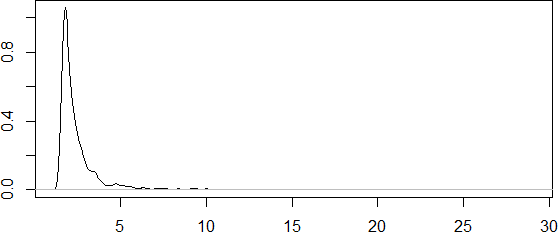
\includegraphics[width=0.75\textwidth]{rytgaard1990/predictive_Y_f.png}
\end{figure}

The draws of \( S_f \), representing a future observation of \( S_t \), were generated as follows:

\begin{enumerate}
\item 1,000 values of \( N_f \) were drawn using the inverse CDF method\footnote{Once again, 1,000 values \( U \sim \mathrm{Uniform}(0, 1) \) were generated. For each value, Poisson samples were drawn for each \( \theta^{(i)} \) using~the inverse CDF method. The results were averaged across \( i \) and rounded to produce 1,000 integer values.}.
\item For each simulated value of \( N_f \), the corresponding number of \( Y_f \) values was drawn using the same procedure as in the predictive PDF estimation, and these values were then summed to generate a draw of \( S_f \).
\end{enumerate}

\noindent Figure~\ref{fig:10} presents the histogram of the resulting \( S_f \) samples, along with three fitted distributions using moment matching. As observed by \citet{dudley2006bayesian}, the Gamma distribution provides the best fit. The fitted Gamma~dis- tribution has parameters \( \alpha = 1.726 \) and \( \beta = 0.202 \).

\begin{figure}[!ht]
\centering
\caption{Histogram and Fitted Distributions for Predictive \( S_f \)}
\label{fig:10}
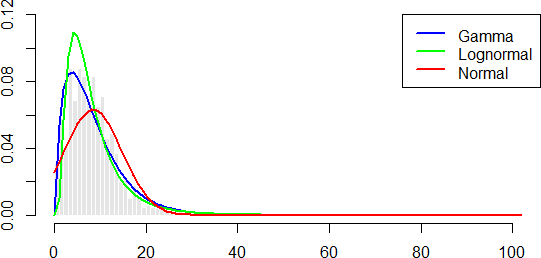
\includegraphics[width=0.75\textwidth]{rytgaard1990/predictive_S_f.png}
\end{figure}

Table~\ref{tab:7} reports various percentiles of the simulated \( S_f \) values. The maximum value of 116.396 reflects~a long tail, consistent with expectations for a heavy-tailed claim size distribution. This indicates that the~simulation ef- fectively captured the tail behavior of the predictive distribution of \( S \), which is important since most aggregate claims are moderate, but extreme values can occasionally occur.

\begin{table}[!ht]
\centering
\footnotesize
\setlength{\tabcolsep}{5pt}
\caption{Percentiles of Simulated \( S_f \) Values}
\label{tab:7}
\begin{tabular}{
>{\raggedright\arraybackslash}p{\widthof{99th Percentile}}
S[table-format=3.3]
}
\hline
\textbf{Percentile} & \textbf{Value} \\ 
\hline
Median & 7.504 \\ 
90th Percentile & 15.065 \\
95th Percentile & 18.092 \\
99th Percentile & 25.171 \\
Maximum & 116.396 \\
\hline
\end{tabular}
\end{table}

\section{Implementation on Alternative Data}

To assess the generalizability of the Bayesian approach proposed by \citet{dudley2006bayesian} for insurance claim modeling, the same methodology was applied to a different dataset. The \texttt{itamtplcost} dataset consists of 457 motor~insur- ance claims exceeding 500{,}000 euros, recorded in Italy between 1997 and 2012 \citep{Dutang2020}.

Table~\ref{tab:8} compares summary statistics between the \citet{rytgaard1990pareto} and \texttt{itamtplcost} datasets. Claims in the \texttt{itamtplcost} dataset are substantially larger, with a mean of 1.015~billion euros compared to 3.058~million euros in the \citet{rytgaard1990pareto} dataset. The variability is also markedly higher, with a range of 6{,}637.34 versus 17.56. In terms of annual claim counts, the \texttt{itamtplcost} dataset spans from 5 to 40 claims per year, whereas the \citet{rytgaard1990pareto} dataset ranges from 0 to 5. These differences underscore the greater complexity of the \texttt{itamtplcost}~data- set, offering a meaningful test of whether the Poisson--Pareto model can still yield valid~posterior inference~in~a more realistic insurance context.

\begin{table}[!ht]
\centering
\footnotesize
\setlength{\tabcolsep}{5pt}
\caption{Comparison of Summary Statistics Between Datasets}
\label{tab:8}
\begin{tabular}{
>{\raggedright\arraybackslash}p{\widthof{\citet{rytgaard1990pareto}}}
*{6}{S[table-format=4.3]}
}
\hline
\textbf{Dataset} & \textbf{Min} & \textbf{1st Qu.} & \textbf{Median} & \textbf{Mean} & \textbf{3rd Qu.} & \textbf{Max} \\
\hline
& \multicolumn{6}{c}{\textbf{Claim Amounts (in millions)}} \\
\hline
\citet{rytgaard1990pareto} & 1.625 & 1.745 & 1.863 & 3.058 & 2.109 & 19.180 \\
\texttt{itamtplcost} & 2.161 & 627.719 & 844.011 & 1015.352 & 1224.316 & 6639.500 \\
\hline
& \multicolumn{6}{c}{\textbf{Claim Counts}} \\
\hline
\citet{rytgaard1990pareto} & 0.00 & 3.00 & 4.00 & 3.20 & 4.00 & 5.00 \\
\texttt{itamtplcost} & 5.00 & 24.25 & 30.50 & 28.56 & 35.25 & 40.00 \\
\hline
\end{tabular}
\end{table}

\subsection{Poisson--Pareto Model}

As previously, Gibbs sampling was employed to generate samples from the posterior distributions of \(\alpha\), \(\beta\), and \(\theta\), with three Markov chains run in parallel using well-dispersed initial parameter values. An initial burn-in~of~1{,}000 iterations was applied. However, the Gelman--Rubin diagnostic \citeyearpar{Gelman1992} indicated that a longer burn-in period was necessary. Accordingly, the burn-in was extended to 10{,}000 iterations. Autocorrelation plots revealed substan- tial autocorrelation in the samples, particularly for certain parameters, prompting the use of a thinning interval of 10. The chains were rerun with this setting, and the resulting trace and autocorrelation plots demonstrated good mixing and negligible autocorrelation across all lags.

Despite this, all simulated values of \(\alpha\) were below 1, indicating that the mean of the Pareto distribution~was infinite. This posed a risk of instability in the results and led to the conclusion that the Poisson--Pareto model was not suitable for the \texttt{itamtplcost} dataset. Consequently, alternative loss distributions were considered,~including the Weibull and Lognormal. Of these, the Lognormal distribution was preferred, as it yields a heavier tail in~the predictive distribution of \( S_f \), which is more appropriate given the presence---albeit rare---of extremely large~ag- gregate claims.

In addition, alternatives to the Poisson distribution for modeling claim counts were considered, as the~empirical mean and variance of \( N_t \)—28.563 and 90.529, respectively—differed substantially, indicating a likely~violation of the Poisson assumption of equality between mean and variance. This contrasts with the \citet{rytgaard1990pareto}~da- taset, where the sample mean and variance were more closely aligned (3.2 vs.\ 3.7). Both the Poisson and~Negative Binomial distributions provided a reasonable fit to the data. Accordingly, two models are reported below:\ the Poisson--Lognormal and the Negative Binomial--Lognormal.

\subsection{Poisson--Lognormal Model}

The Lognormal distribution was parameterized in terms of \( \mu \) and \( \tau \), where \( \tau = 1 / \sigma^2 \). A vague Normal prior was assigned to \( \mu \), and vague Gamma priors were used for both \( \sigma \) and \( \theta \). As in previous models, three Markov chains were run in parallel with well-dispersed initial parameter values. For the third chain, initial values were~set~equal to the maximum likelihood estimates (see Table~\ref{tab:9}).

\begin{table}[!ht]
\centering
\footnotesize
\setlength{\tabcolsep}{5pt}
\caption{Initial Parameter Values}
\label{tab:9}
\begin{tabular}{
>{\raggedright\arraybackslash}p{\widthof{Chain}}
*{3}{S[table-format=6.5]}
}
\hline
\textbf{Chain} & \( \mu \) & \( \sigma \) & \( \theta \) \\ \hline
1 & 0.00001 & 0.00001 & 0.00001 \\
2 & 100000 & 100000 & 100000 \\
3 & 6.700 & 0.802 & 28.563 \\ \hline
\end{tabular}
\end{table}

An initial burn-in of 1{,}000 iterations was applied. However, the Gelman--Rubin diagnostic (\citeyear{Gelman1992}) suggested that this was insufficient, as convergence had not yet been achieved. The PSRF point estimates stabilized~around 1 only after approximately 10{,}000 iterations, which was then adopted as the revised burn-in. Moderate~autocor- relation was observed in the chains, prompting the use of a thinning interval of 10. The chains were rerun with this setting, and updated diagnostics showed negligible autocorrelation across all lags. Trace plots of the~param- eters, shown in Figure~\ref{fig:13}, support the conclusion of good mixing and convergence.

\begin{figure}[!ht]
    \centering
    \caption{Trace Plots After Thinning}
    \label{fig:13}
    \begin{subfigure}{0.45\textwidth}
        \centering
        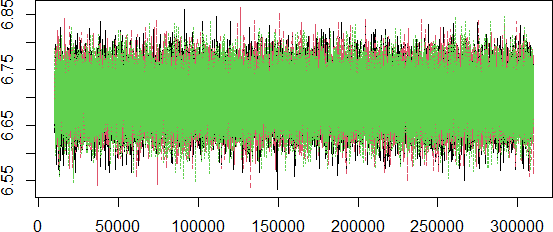
\includegraphics[width=\textwidth]{itamtplcost/trace_after_thinning_mu.png}
        \caption{\( \mu \)}
    \end{subfigure}
    \hfill
    \begin{subfigure}{0.45\textwidth}
        \centering
        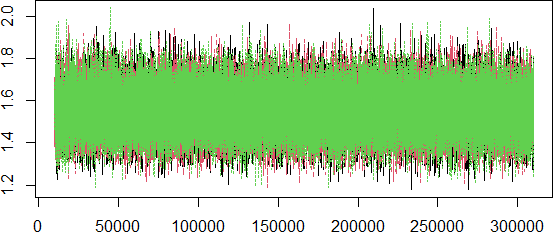
\includegraphics[width=\textwidth]{itamtplcost/trace_after_thinning_tau.png}
        \caption{\( \tau \)}
    \end{subfigure}

    \vspace{1em}

    \begin{subfigure}{0.45\textwidth}
        \centering
        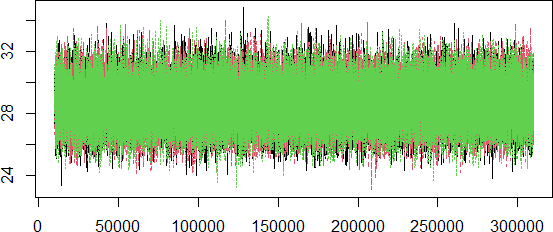
\includegraphics[width=\textwidth]{itamtplcost/trace_after_thinning_theta.png}
        \caption{\( \theta \)}
    \end{subfigure}
\end{figure}

Table~\ref{tab:11} reports posterior summary statistics based on 30{,}000 post-burn-in samples. The posterior means~are closely aligned with the maximum likelihood estimates (MLE)\footnote{The MLE for \( \tau \) is 1.554.}, as expected under vague priors, since the inference is primarily driven by the data. The sample mean of \( Y \), equal to 1{,}015.352, lies within the Bayesian credible interval for \( \mathbb{E}[Y] \). The posterior mean of \( \mathbb{E}[Y] \) is slightly higher, reflecting the influence of several extremely~large claim amounts (exceeding 3~billion euros). Compared to the results from the \citet{rytgaard1990pareto} dataset, the 95\% credible intervals are narrower or of comparable width, indicating good estimation precision—likely due to the larger sample size.

\begin{table}[!ht]
\centering
\footnotesize
\setlength{\tabcolsep}{5pt}
\caption{Posterior Statistics}
\label{tab:11}
\begin{tabular}{
>{\raggedright\arraybackslash}p{\widthof{\( \mathbb{E}[y] \)}}
*{2}{S[table-format=4.3]}
>{\raggedright\arraybackslash}p{\widthof{\textbf{95\% Bayesian Credible Interval}}}
}
\hline
 & \textbf{Mean} & \textbf{Standard Deviation} & \textbf{95\% Bayesian Credible Interval} \\ \hline
\( \mu \) & 6.700 & 0.038 & (6.626, 6.774) \\
\( \tau \) & 1.552 & 0.103 & (1.358, 1.759) \\
\( \theta \) & 28.628 & 1.337 & (26.058, 31.313) \\
\( \mathbb{E}[y] \) & 1124.280 & 48.873 & (1034.404, 1225.412) \\ \hline
\end{tabular}
\end{table}

Figure~\ref{fig:15} shows the posterior density plots for \( \mu \), \( \tau \), and \( \theta \). The posterior for \( \mu \) appears approximately~Normal, while the distributions of \( \tau \) and \( \theta \) resemble Gamma distributions. The posterior for \( \mathbb{E}[Y] \) is right-skewed, though notably less so than in the \citet{rytgaard1990pareto} dataset.

\begin{figure}[!ht]
    \centering
    \caption{Posterior Densities}
    \label{fig:15}
    \begin{minipage}{0.45\textwidth}
        \centering
        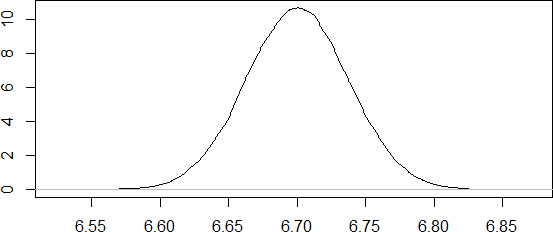
\includegraphics[width=\textwidth]{itamtplcost/density_mu.png}
        \subcaption{\( \mu \)}
    \end{minipage}%
    \hfill
    \begin{minipage}{0.45\textwidth}
        \centering
        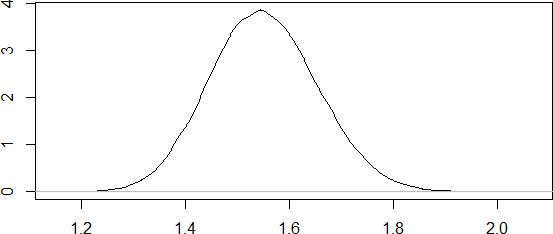
\includegraphics[width=\textwidth]{itamtplcost/density_tau.png}
        \subcaption{\( \tau \)}
    \end{minipage} \\
    
    \vspace{0.5cm}
    
    \begin{minipage}{0.45\textwidth}
        \centering
        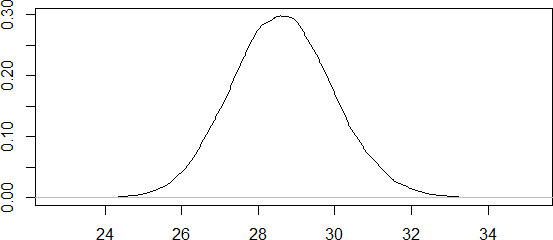
\includegraphics[width=\textwidth]{itamtplcost/density_theta.png}
        \subcaption{\( \theta \)}
    \end{minipage}%
    \hfill
    \begin{minipage}{0.45\textwidth}
        \centering
        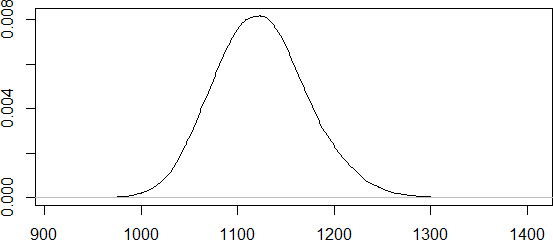
\includegraphics[width=\textwidth]{itamtplcost/density_E_y.png}
        \subcaption{\( \mathbb{E}[y] \)}
    \end{minipage}
    
\end{figure}

Figure~\ref{fig:16} compares the empirical cumulative distribution of observed claim amounts \( y_{i,t} \) with the cumulative distribution function (CDF) of a Lognormal distribution parameterized by the posterior means of \( \mu \) and~\( \tau \). The Lognormal\((6.700,\,1.552)\) distribution closely matches the empirical data. Figure~\ref{fig:17} presents a~similar comparison for the claim frequency data \( n_t \), evaluated against the CDF of a Poisson distribution with mean equal to the posterior mean of \( \theta \). The Poisson\((28.628)\) distribution captures the overall trend of the empirical~distribution well, though there is room for improvement.

\begin{figure}[!ht]
    \centering
    \caption{Empirical vs.\ Fitted Lognormal CDF}
    \label{fig:16}
    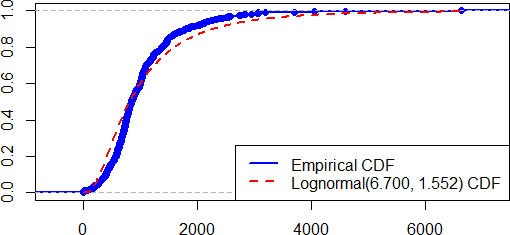
\includegraphics[width=.75\textwidth]{itamtplcost/empirical_vs_lognormal.png}
\end{figure}

\begin{figure}[!ht]
    \centering
    \caption{Empirical vs.\ Fitted Poisson CDF}
    \label{fig:17}
    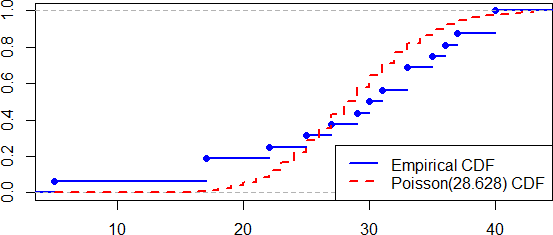
\includegraphics[width=.75\textwidth]{itamtplcost/empirical_vs_poisson.png}
\end{figure}

Figure~\ref{fig:18} displays the estimated predictive probability density function (PDF) of a future individual claim amount \( Y_f \), obtained using the inverse CDF method, similarly as in the previous section. The resulting~distribu- tion is markedly right-skewed, capturing the heavy-tailed nature of claim sizes. While extremely large values~are possible, they occur with very low probability.

\begin{figure}[!ht]
\centering
\caption{Estimated Predictive PDF of \( Y_f \) }
\label{fig:18}
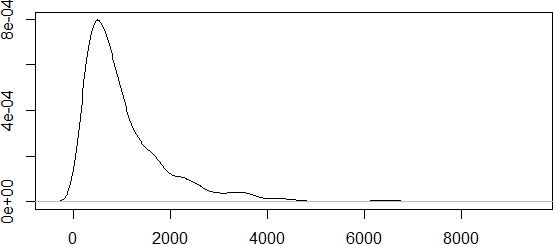
\includegraphics[width=0.75\textwidth]{itamtplcost/predictive_Y_f.png}
\end{figure}

Finally, Figure~\ref{fig:19} presents the histogram of simulated aggregate claims \( S_f \), obtained using the same predictive simulation approach as in the previous section. Three theoretical distributions were fitted to the simulated values using moment matching. Among these, the Gamma distribution appears to provide the best fit, with~esti- mated parameters \( \alpha = 15.6920 \) and \( \beta = 0.0005 \).

\begin{figure}[!ht]
\centering
\caption{Histogram and Fitted Distributions for Predictive \( S_f \)}
\label{fig:19}
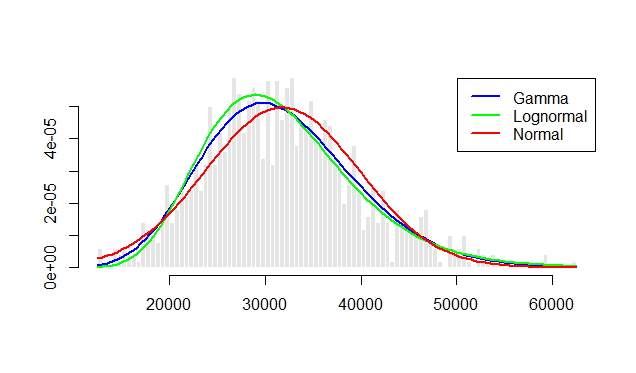
\includegraphics[width=0.75\textwidth]{itamtplcost/predictive_S_f.png}
\end{figure}

\subsection{Negative Binomial--Lognormal Model}

As previously noted, upon examining the sample mean and variance of claim counts in the \texttt{itamtplcost} dataset, it became apparent that the Poisson assumption, which assumes equality between the mean and variance of~\( N_t \), was likely violated. As a result, an alternative distribution for modeling claim counts was explored. The~Negative Binomial distribution is commonly used when overdispersion is present in count data, meaning the variance~ex- ceeds the mean.

The Negative Binomial distribution was parameterized in terms of \( r \) and \( p \), where \( r \) represents the number~of successes required before an experiment is stopped, and \( p \) is the probability of success in each trial. A vague~Beta prior was assigned to \( p \), as it must lie between 0 and 1, while a vague Gamma prior was used for \( r \), as \( r \) can~take any positive real value. Three Markov chains were run in parallel with varied initial parameter values, as~summa- rized in Table~\ref{tab:12}.

\begin{table}[!ht]
\centering
\footnotesize
\setlength{\tabcolsep}{5pt}
\caption{Initial Parameter Values}
\label{tab:12}
\begin{tabular}{
>{\raggedright\arraybackslash}p{\widthof{Chain}}
*{4}{S[table-format=2.3]}
}
\hline
\textbf{Chain} & \( \mu \) & \( \sigma \) & \( r \) & \( p \) \\ \hline
1 & 0.01 & 0.50 & 5.00 & 0.20 \\
2 & 2.0 & 1.5 & 10.0 & 0.5 \\
3 & 6.700 & 0.802 & 13.165 & 0.316 \\ \hline
\end{tabular}
\end{table}

As previously, the burn-in period was initially set to 1,000 iterations, and the PSRF point estimates were~examined to determine if this duration was sufficient. The plots indicated that a burn-in of 20,000 iterations was necessary, so the chains were rerun with this setting. Autocorrelation values for lags 1 through 10 were computed, revealing significant autocorrelations, particularly for \( r \) and \( p \), with values reaching as high as 0.9. Consequently, a thinning interval of 10 was insufficient, and a thinning interval of 100 was applied. This adjustment effectively reduced autocorrelation, and the resulting trace plots (Figure~\ref{fig:20}) indicated good mixing and convergence.

\begin{figure}[!ht]
    \centering
    \caption{Trace Plots After Thinning}
    \label{fig:20}
    \begin{subfigure}{0.45\textwidth}
        \centering
        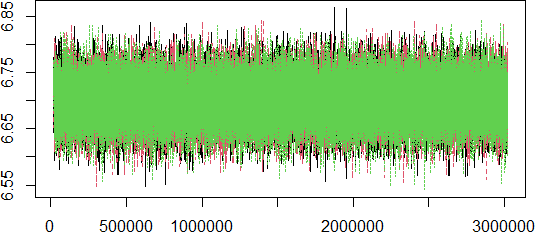
\includegraphics[width=\textwidth]{itamtplcost_nb/trace_after_thinning_mu.png}
        \caption{\( \mu \)}
    \end{subfigure}
    \hfill
    \begin{subfigure}{0.45\textwidth}
        \centering
        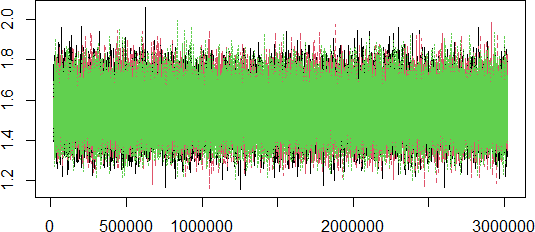
\includegraphics[width=\textwidth]{itamtplcost_nb/trace_after_thinning_tau.png}
        \caption{\( \tau \)}
    \end{subfigure}

    \vspace{1em}

    \begin{subfigure}{0.45\textwidth}
        \centering
        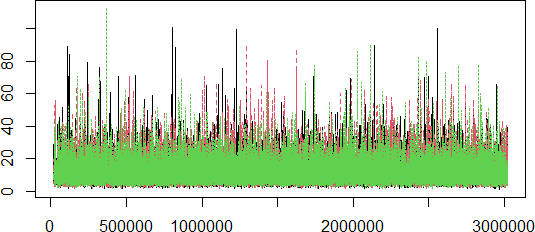
\includegraphics[width=\textwidth]{itamtplcost_nb/trace_after_thinning_r.png}
        \caption{\( r \)}
    \end{subfigure}
    \hfill
    \begin{subfigure}{0.45\textwidth}
        \centering
        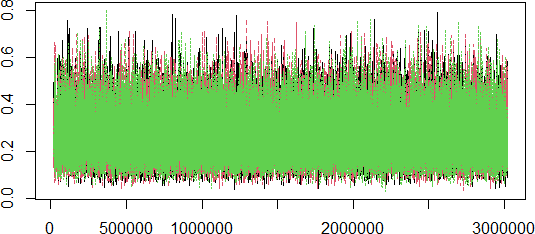
\includegraphics[width=\textwidth]{itamtplcost_nb/trace_after_thinning_p.png}
        \caption{\( p \)}
    \end{subfigure}
\end{figure}

Table~\ref{tab:13} shows posterior summary statistics based on 30{,}000 post-burn-in iterations. The estimates for \( \mu \) and \( \tau \) closely match those obtained in the Poisson--Lognormal model, providing further confirmation of convergence for these parameters. Figure~\ref{fig:21} displays posterior density plots for \( r \) and \( p \). As expected, the posterior distri- bution of \( r \) resembles a Gamma distribution, while that of \( p \) aligns with a Beta distribution--appropriately con- strained to the \([0, 1]\) interval.

\begin{table}[!ht]
\centering
\footnotesize
\setlength{\tabcolsep}{5pt}
\caption{Posterior Statistics}
\label{tab:13}
\begin{tabular}{
>{\raggedright\arraybackslash}p{\widthof{\( \mathbb{E}[y] \)}}
*{2}{S[table-format=4.3]}
>{\raggedright\arraybackslash}p{\widthof{\textbf{95\% Bayesian Credible Interval}}}
}
\hline
 & \textbf{Mean} & \textbf{Standard Deviation} & \textbf{95\% Bayesian Credible Interval} \\ \hline
\( \mu \) & 6.700 & 0.038 & (6.627, 6.774) \\
\( \tau \) & 1.551 & 0.103 & (1.355, 1.759) \\
\( r \) & 11.229 & 6.619 & (3.690, 27.960) \\
\( p \) & 0.267 & 0.099 & (0.112, 0.497) \\
\( \mathbb{E}[y] \) & 1124.596 & 49.010 & (1034.370, 1226.564) \\ \hline
\end{tabular}
\end{table}

\begin{figure}[!ht]
    \centering
    \caption{Posterior Densities}
    \label{fig:21}
    \begin{minipage}{0.45\textwidth}
        \centering
        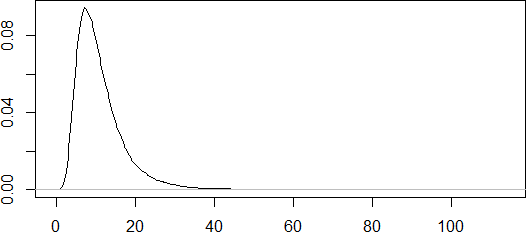
\includegraphics[width=\textwidth]{itamtplcost_nb/density_r.png}
        \subcaption{\( r \)}
    \end{minipage}%
    \hfill
    \begin{minipage}{0.45\textwidth}
        \centering
        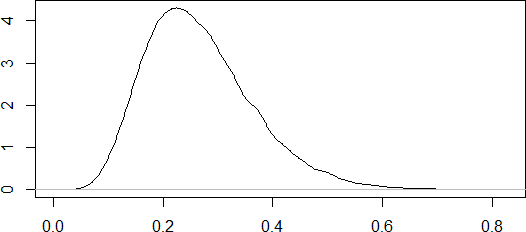
\includegraphics[width=\textwidth]{itamtplcost_nb/density_p.png}
        \subcaption{\( p \)}
    \end{minipage} \\
    
\end{figure}

Figure~\ref{fig:22} compares the empirical cumulative distribution function (ECDF) of the observed claim counts \( n_t \) with the CDF of a Negative Binomial distribution parameterized by the posterior means of \( r \) and \( p \). The fitted distribution closely follows the ECDF in the central region, although it converges more slowly toward 1.

\begin{figure}[!ht]
    \centering
    \caption{Empirical vs.\ Fitted Negative Binomial CDF}
    \label{fig:22}
    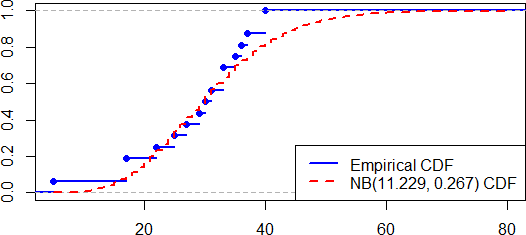
\includegraphics[width=.75\textwidth]{itamtplcost_nb/empirical_vs_nb.png}
\end{figure}

Finally, Figure~\ref{fig:23} presents the histogram of simulated aggregate claims \( S_f \), with three distributions fitted~via moment matching. Once again, the Gamma distribution appears to provide the best approximation to the~dis- tribution of aggregate claims, with estimated parameters \( \alpha = 5.48143 \) and \( \beta = 0.00017 \).

\begin{figure}[!ht]
\centering
\caption{Histogram and Fitted Distributions for Predictive \( S_f \)}
\label{fig:23}
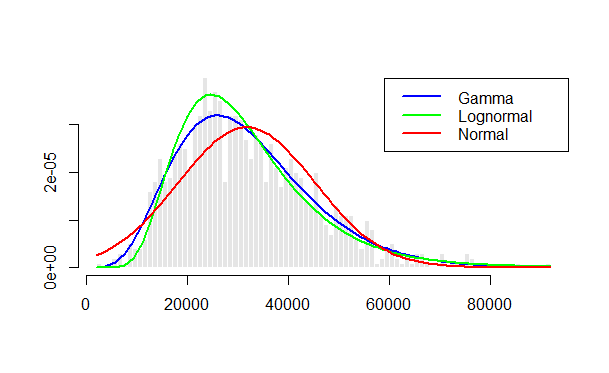
\includegraphics[width=0.75\textwidth]{itamtplcost_nb/predictive_S_f.png}
\end{figure}

Table~\ref{tab:14} compares various percentiles of the simulated \( S_f \) values for the two models:\ Poisson--Lognormal and Negative Binomial--Lognormal. With maxima of 62{,}054.06 and 91{,}825.33, respectively, both models effectively capture the heavy tail of the predictive distribution of \( S_f \). However, the Negative Binomial--Lognormal model provides a slightly better fit in the tail, as indicated by its higher maximum. This difference is also evident~when comparing Figures~\ref{fig:19} and~\ref{fig:23}.

\begin{table}[!ht]
\centering
\footnotesize
\setlength{\tabcolsep}{5pt}
\caption{Comparison of Percentiles of Simulated \( S_f \) Values for Two Models}
\label{tab:14}
\begin{tabular}{
>{\raggedright\arraybackslash}p{\widthof{99th Percentile}}
S[table-format=5.2]
S[table-format=5.2]
}
\hline
\textbf{Percentile} & \textbf{Poisson--Lognormal} & \textbf{Negative Binomial--Lognormal} \\
\hline
Median & 31278.27 & 29538.01 \\ 
90th Percentile & 42380.49 & 50239.35 \\
95th Percentile & 46347.16 & 55750.20 \\
99th Percentile & 52800.55 & 73525.82 \\
Maximum & 62054.06 & 91825.33 \\
\hline
\end{tabular}
\end{table}

The improved tail behavior is due to the additional dispersion allowed by the Negative Binomial distribution in modeling claim counts, in contrast to the more restrictive Poisson distribution. Table~\ref{tab:15} presents a comparison of summary statistics for the simulated values of \( N_f \) under both models. Although the means of the simulated values are nearly identical, the~values for the Poisson distribution range from 13 to 47, while those for the~Nega- tive Binomial range from 4 to 76.

\begin{table}[!ht]
\centering
\footnotesize
\setlength{\tabcolsep}{10pt}
\caption{Comparison of Summary Statistics for Claim Count Models}
\label{tab:15}
\begin{tabular}{
>{\raggedright\arraybackslash}p{\widthof{Negative Binomial}} 
*{6}{S[table-format=2.2]}
}
\hline
\textbf{Model} & \textbf{Min.} & \textbf{1st Qu.} & \textbf{Median} & \textbf{Mean} & \textbf{3rd Qu.} & \textbf{Max.} \\ 
\hline
Poisson & 13.00 & 25.00 & 28.00 & 28.56 & 32.00 & 47.00 \\
Negative Binomial & 4.00 & 21.00 & 27.00 & 28.50 & 35.00 & 76.00 \\
\hline
\end{tabular}
\end{table}


\printbibliography{references}
\end{document}